\documentclass{extbook}[14pt]
\usepackage{multicol, enumerate, enumitem, hyperref, color, soul, setspace, parskip, fancyhdr, amssymb, amsthm, amsmath, bbm, latexsym, units, mathtools}
\everymath{\displaystyle}
\usepackage[headsep=0.5cm,headheight=0cm, left=1 in,right= 1 in,top= 1 in,bottom= 1 in]{geometry}
\usepackage{dashrule}  % Package to use the command below to create lines between items
\newcommand{\litem}[1]{\item #1

\rule{\textwidth}{0.4pt}}
\pagestyle{fancy}
\lhead{}
\chead{Answer Key for Progress Quiz 3 Version C}
\rhead{}
\lfoot{3148-2249}
\cfoot{}
\rfoot{Spring 2021}
\begin{document}
\textbf{This key should allow you to understand why you choose the option you did (beyond just getting a question right or wrong). \href{https://xronos.clas.ufl.edu/mac1105spring2020/courseDescriptionAndMisc/Exams/LearningFromResults}{More instructions on how to use this key can be found here}.}

\textbf{If you have a suggestion to make the keys better, \href{https://forms.gle/CZkbZmPbC9XALEE88}{please fill out the short survey here}.}

\textit{Note: This key is auto-generated and may contain issues and/or errors. The keys are reviewed after each exam to ensure grading is done accurately. If there are issues (like duplicate options), they are noted in the offline gradebook. The keys are a work-in-progress to give students as many resources to improve as possible.}

\rule{\textwidth}{0.4pt}

\begin{enumerate}\litem{
Construct the lowest-degree polynomial given the zeros below. Then, choose the intervals that contain the coefficients of the polynomial in the form $x^3+bx^2+cx+d$.
\[ -2 - 5 i \text{ and } -3 \]

The solution is \( x^{3} +7 x^{2} +41 x + 87 \), which is option C.\begin{enumerate}[label=\Alph*.]
\item \( b \in [-13, -2], c \in [40, 42.8], \text{ and } d \in [-90, -77] \)

$x^{3} -7 x^{2} +41 x -87$, which corresponds to multiplying out $(x-(-2 - 5 i))(x-(-2 + 5 i))(x -3)$.
\item \( b \in [-3, 2], c \in [3.1, 6.1], \text{ and } d \in [-1, 8] \)

$x^{3} + x^{2} +5 x + 6$, which corresponds to multiplying out $(x + 2)(x + 3)$.
\item \( b \in [6, 10], c \in [40, 42.8], \text{ and } d \in [84, 96] \)

* $x^{3} +7 x^{2} +41 x + 87$, which is the correct option.
\item \( b \in [-3, 2], c \in [5.5, 10.3], \text{ and } d \in [13, 21] \)

$x^{3} + x^{2} +8 x + 15$, which corresponds to multiplying out $(x + 5)(x + 3)$.
\item \( \text{None of the above.} \)

This corresponds to making an unanticipated error or not understanding how to use nonreal complex numbers to create the lowest-degree polynomial. If you chose this and are not sure what you did wrong, please contact the coordinator for help.
\end{enumerate}

\textbf{General Comment:} Remember that the conjugate of $a+bi$ is $a-bi$. Since these zeros always come in pairs, we need to multiply out $(x-(-2 - 5 i))(x-(-2 + 5 i))(x-(-3))$.
}
\litem{
Construct the lowest-degree polynomial given the zeros below. Then, choose the intervals that contain the coefficients of the polynomial in the form $ax^3+bx^2+cx+d$.
\[ \frac{-3}{2}, \frac{-5}{4}, \text{ and } \frac{7}{4} \]

The solution is \( 32x^{3} +32 x^{2} -94 x -105 \), which is option B.\begin{enumerate}[label=\Alph*.]
\item \( a \in [26, 33], b \in [-38, -30], c \in [-101, -92], \text{ and } d \in [105, 110] \)

$32x^{3} -32 x^{2} -94 x + 105$, which corresponds to multiplying out $(2x -3)(4x -5)(4x + 7)$.
\item \( a \in [26, 33], b \in [32, 36], c \in [-101, -92], \text{ and } d \in [-111, -104] \)

* $32x^{3} +32 x^{2} -94 x -105$, which is the correct option.
\item \( a \in [26, 33], b \in [32, 36], c \in [-101, -92], \text{ and } d \in [105, 110] \)

$32x^{3} +32 x^{2} -94 x + 105$, which corresponds to multiplying everything correctly except the constant term.
\item \( a \in [26, 33], b \in [-144, -138], c \in [207, 217], \text{ and } d \in [-111, -104] \)

$32x^{3} -144 x^{2} +214 x -105$, which corresponds to multiplying out $(2x -3)(4x -5)(4x -7)$.
\item \( a \in [26, 33], b \in [-72, -58], c \in [-56, -45], \text{ and } d \in [105, 110] \)

$32x^{3} -64 x^{2} -46 x + 105$, which corresponds to multiplying out $(2x -3)(4x + 5)(4x -7)$.
\end{enumerate}

\textbf{General Comment:} To construct the lowest-degree polynomial, you want to multiply out $(2x + 3)(4x + 5)(4x -7)$
}
\litem{
Which of the following equations \textit{could} be of the graph presented below?

\begin{center}
    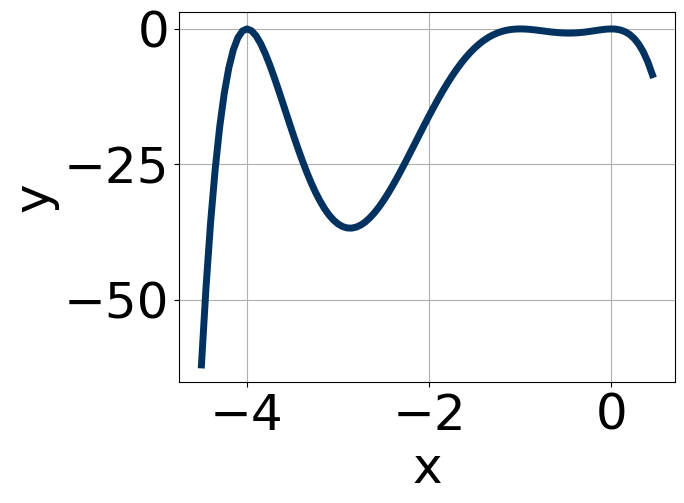
\includegraphics[width=0.5\textwidth]{../Figures/polyGraphToFunctionC.png}
\end{center}




The solution is \( 12x^{10} (x + 3)^{9} (x - 2)^{11} \), which is option B.\begin{enumerate}[label=\Alph*.]
\item \( -13x^{6} (x + 3)^{7} (x - 2)^{10} \)

The factor $(x - 2)$ should have an odd power and the leading coefficient should be the opposite sign.
\item \( 12x^{10} (x + 3)^{9} (x - 2)^{11} \)

* This is the correct option.
\item \( -3x^{6} (x + 3)^{5} (x - 2)^{5} \)

This corresponds to the leading coefficient being the opposite value than it should be.
\item \( 15x^{7} (x + 3)^{10} (x - 2)^{5} \)

The factor $0$ should have an even power and the factor $-3$ should have an odd power.
\item \( 19x^{10} (x + 3)^{8} (x - 2)^{9} \)

The factor $(x + 3)$ should have an odd power.
\end{enumerate}

\textbf{General Comment:} General Comments: Draw the x-axis to determine which zeros are touching (and so have even multiplicity) or cross (and have odd multiplicity).
}
\litem{
Describe the end behavior of the polynomial below.
\[ f(x) = 7(x - 9)^{5}(x + 9)^{8}(x + 2)^{4}(x - 2)^{4} \]

The solution is the graph below, which is option D.
\begin{center}
    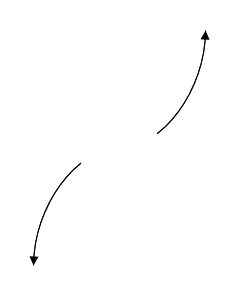
\includegraphics[width=0.3\textwidth]{../Figures/polyEndBehaviorCopyDC.png}
\end{center}\begin{enumerate}[label=\Alph*.]
\begin{multicols}{2}
\item 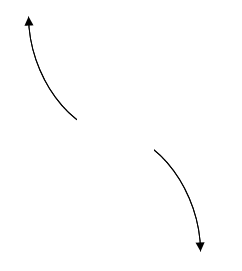
\includegraphics[width = 0.3\textwidth]{../Figures/polyEndBehaviorCopyAC.png}
\item 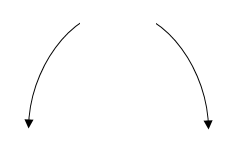
\includegraphics[width = 0.3\textwidth]{../Figures/polyEndBehaviorCopyBC.png}
\item 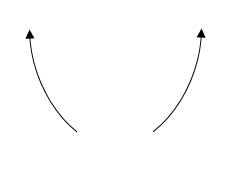
\includegraphics[width = 0.3\textwidth]{../Figures/polyEndBehaviorCopyCC.png}
\item 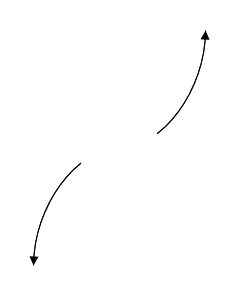
\includegraphics[width = 0.3\textwidth]{../Figures/polyEndBehaviorCopyDC.png}
\end{multicols}\item None of the above.\end{enumerate}
\textbf{General Comment:} Remember that end behavior is determined by the leading coefficient AND whether the \textbf{sum} of the multiplicities is positive or negative.
}
\litem{
Construct the lowest-degree polynomial given the zeros below. Then, choose the intervals that contain the coefficients of the polynomial in the form $ax^3+bx^2+cx+d$.
\[ -3, \frac{2}{3}, \text{ and } -7 \]

The solution is \( 3x^{3} +28 x^{2} +43 x -42 \), which is option D.\begin{enumerate}[label=\Alph*.]
\item \( a \in [3, 5], b \in [-28.7, -25.9], c \in [42, 48], \text{ and } d \in [41, 44] \)

$3x^{3} -28 x^{2} +43 x + 42$, which corresponds to multiplying out $(x -3)(3x + 2)(x -7)$.
\item \( a \in [3, 5], b \in [13.4, 15.1], c \in [-56, -54], \text{ and } d \in [-42, -41] \)

$3x^{3} +14 x^{2} -55 x -42$, which corresponds to multiplying out $(x -3)(3x + 2)(x + 7)$.
\item \( a \in [3, 5], b \in [6.1, 12.1], c \in [-75, -70], \text{ and } d \in [41, 44] \)

$3x^{3} +10 x^{2} -71 x + 42$, which corresponds to multiplying out $(x -3)(3x -2)(x + 7)$.
\item \( a \in [3, 5], b \in [27.6, 30.4], c \in [42, 48], \text{ and } d \in [-42, -41] \)

* $3x^{3} +28 x^{2} +43 x -42$, which is the correct option.
\item \( a \in [3, 5], b \in [27.6, 30.4], c \in [42, 48], \text{ and } d \in [41, 44] \)

$3x^{3} +28 x^{2} +43 x + 42$, which corresponds to multiplying everything correctly except the constant term.
\end{enumerate}

\textbf{General Comment:} To construct the lowest-degree polynomial, you want to multiply out $(x + 3)(3x -2)(x + 7)$
}
\litem{
Which of the following equations \textit{could} be of the graph presented below?

\begin{center}
    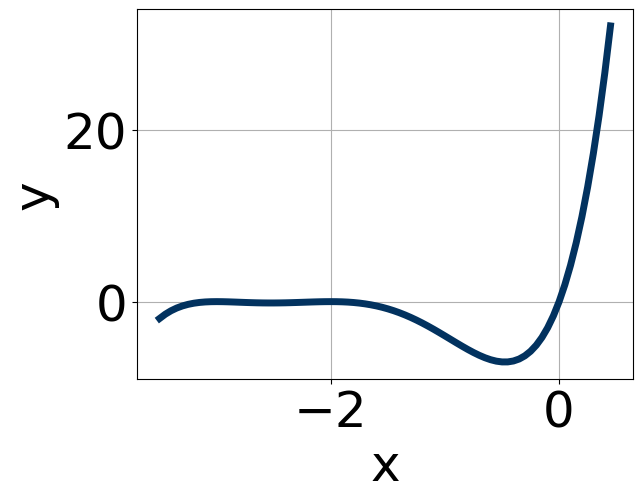
\includegraphics[width=0.5\textwidth]{../Figures/polyGraphToFunctionCopyC.png}
\end{center}




The solution is \( 18x^{11} (x + 4)^{4} (x + 3)^{7} \), which is option C.\begin{enumerate}[label=\Alph*.]
\item \( -14x^{5} (x + 4)^{10} (x + 3)^{11} \)

This corresponds to the leading coefficient being the opposite value than it should be.
\item \( -15x^{6} (x + 4)^{8} (x + 3)^{5} \)

The factor $x$ should have an odd power and the leading coefficient should be the opposite sign.
\item \( 18x^{11} (x + 4)^{4} (x + 3)^{7} \)

* This is the correct option.
\item \( 12x^{11} (x + 4)^{10} (x + 3)^{10} \)

The factor $(x + 3)$ should have an odd power.
\item \( 5x^{11} (x + 4)^{9} (x + 3)^{4} \)

The factor $-4$ should have an even power and the factor $-3$ should have an odd power.
\end{enumerate}

\textbf{General Comment:} General Comments: Draw the x-axis to determine which zeros are touching (and so have even multiplicity) or cross (and have odd multiplicity).
}
\litem{
Describe the zero behavior of the zero $x = 7$ of the polynomial below.
\[ f(x) = 3(x - 7)^{8}(x + 7)^{11}(x + 5)^{3}(x - 5)^{4} \]

The solution is the graph below, which is option C.
\begin{center}
    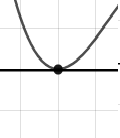
\includegraphics[width=0.3\textwidth]{../Figures/polyZeroBehaviorCC.png}
\end{center}\begin{enumerate}[label=\Alph*.]
\begin{multicols}{2}
\item 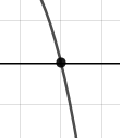
\includegraphics[width = 0.3\textwidth]{../Figures/polyZeroBehaviorAC.png}
\item 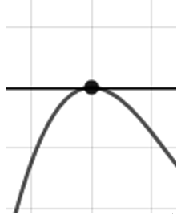
\includegraphics[width = 0.3\textwidth]{../Figures/polyZeroBehaviorBC.png}
\item 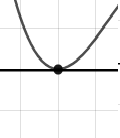
\includegraphics[width = 0.3\textwidth]{../Figures/polyZeroBehaviorCC.png}
\item 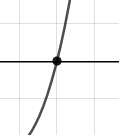
\includegraphics[width = 0.3\textwidth]{../Figures/polyZeroBehaviorDC.png}
\end{multicols}\item None of the above.\end{enumerate}
\textbf{General Comment:} You will need to sketch the entire graph, then zoom in on the zero the question asks about.
}
\litem{
Construct the lowest-degree polynomial given the zeros below. Then, choose the intervals that contain the coefficients of the polynomial in the form $x^3+bx^2+cx+d$.
\[ 4 - 3 i \text{ and } 1 \]

The solution is \( x^{3} -9 x^{2} +33 x -25 \), which is option C.\begin{enumerate}[label=\Alph*.]
\item \( b \in [-4, 3], c \in [1, 7], \text{ and } d \in [-6, -1] \)

$x^{3} + x^{2} +2 x -3$, which corresponds to multiplying out $(x + 3)(x -1)$.
\item \( b \in [-4, 3], c \in [-11, -3], \text{ and } d \in [1, 6] \)

$x^{3} + x^{2} -5 x + 4$, which corresponds to multiplying out $(x -4)(x -1)$.
\item \( b \in [-10, -7], c \in [31, 38], \text{ and } d \in [-25, -20] \)

* $x^{3} -9 x^{2} +33 x -25$, which is the correct option.
\item \( b \in [3, 13], c \in [31, 38], \text{ and } d \in [14, 32] \)

$x^{3} +9 x^{2} +33 x + 25$, which corresponds to multiplying out $(x-(4 - 3 i))(x-(4 + 3 i))(x + 1)$.
\item \( \text{None of the above.} \)

This corresponds to making an unanticipated error or not understanding how to use nonreal complex numbers to create the lowest-degree polynomial. If you chose this and are not sure what you did wrong, please contact the coordinator for help.
\end{enumerate}

\textbf{General Comment:} Remember that the conjugate of $a+bi$ is $a-bi$. Since these zeros always come in pairs, we need to multiply out $(x-(4 - 3 i))(x-(4 + 3 i))(x-(1))$.
}
\litem{
Describe the zero behavior of the zero $x = 7$ of the polynomial below.
\[ f(x) = -8(x - 5)^{10}(x + 5)^{8}(x - 7)^{11}(x + 7)^{6} \]

The solution is the graph below, which is option A.
\begin{center}
    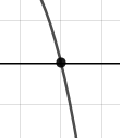
\includegraphics[width=0.3\textwidth]{../Figures/polyZeroBehaviorCopyAC.png}
\end{center}\begin{enumerate}[label=\Alph*.]
\begin{multicols}{2}
\item 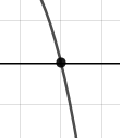
\includegraphics[width = 0.3\textwidth]{../Figures/polyZeroBehaviorCopyAC.png}
\item 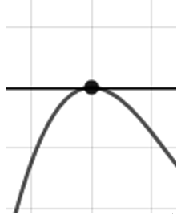
\includegraphics[width = 0.3\textwidth]{../Figures/polyZeroBehaviorCopyBC.png}
\item 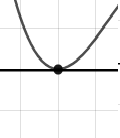
\includegraphics[width = 0.3\textwidth]{../Figures/polyZeroBehaviorCopyCC.png}
\item 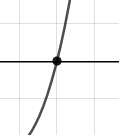
\includegraphics[width = 0.3\textwidth]{../Figures/polyZeroBehaviorCopyDC.png}
\end{multicols}\item None of the above.\end{enumerate}
\textbf{General Comment:} You will need to sketch the entire graph, then zoom in on the zero the question asks about.
}
\litem{
Describe the end behavior of the polynomial below.
\[ f(x) = 8(x + 6)^{5}(x - 6)^{10}(x + 8)^{2}(x - 8)^{2} \]

The solution is the graph below, which is option D.
\begin{center}
    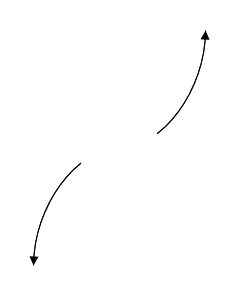
\includegraphics[width=0.3\textwidth]{../Figures/polyEndBehaviorDC.png}
\end{center}\begin{enumerate}[label=\Alph*.]
\begin{multicols}{2}
\item 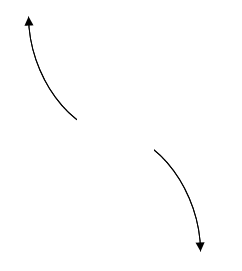
\includegraphics[width = 0.3\textwidth]{../Figures/polyEndBehaviorAC.png}
\item 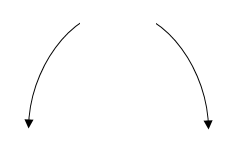
\includegraphics[width = 0.3\textwidth]{../Figures/polyEndBehaviorBC.png}
\item 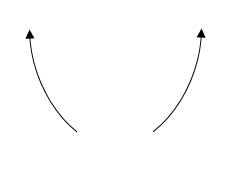
\includegraphics[width = 0.3\textwidth]{../Figures/polyEndBehaviorCC.png}
\item 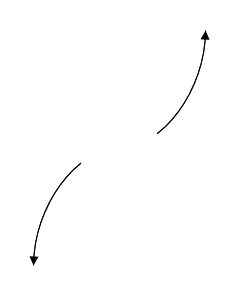
\includegraphics[width = 0.3\textwidth]{../Figures/polyEndBehaviorDC.png}
\end{multicols}\item None of the above.\end{enumerate}
\textbf{General Comment:} Remember that end behavior is determined by the leading coefficient AND whether the \textbf{sum} of the multiplicities is positive or negative.
}
\end{enumerate}

\end{document}